\documentclass[serif, 12pt]{beamer}

\usepackage{graphicx} % Allows including images
\usepackage{booktabs} % Allows the use of \toprule, \midrule and \bottomrule in tables

\usepackage{color}

%\usepackage{algorithm2e}
\usepackage{hyperref}
\usepackage{algorithm,algorithmic}
\usepackage{changepage}

\newcommand*\mat[1]{ \begin{pmatrix} #1 \end{pmatrix}}
\newcommand*\arr[1]{ \begin{bmatrix} #1 \end{bmatrix}}
\newcommand*\V[1]{ \boldsymbol{#1}}

\newcommand*\D{\textcolor{violet}{D}}
\newcommand*\T{\textcolor{blue}{T}}

\setbeamertemplate{navigation symbols}{}%remove navigation symbols

\setbeamerfont{page number in head/foot}{size=\small}
\setbeamertemplate{footline}[frame number]

\title{Approximated PCA}
\subtitle{Iteration 2}

\author{Rodrigo Arias} % Your name
\date{\today} % Date, can be changed to a custom date

\begin{document}

\begin{frame}
	\titlepage
\end{frame}

%------------------------------------------------

\begin{frame}

\frametitle{Computing eigenvalues and eigenvectors}

\begin{enumerate}
\item Take the $n\times n$ target matrix $A = S$.
\item Compute a \textcolor{blue}{tridiagonal} matrix $\T$: $A = P \T P^T$.
\item From $\T$ compute a \textcolor{violet}{diagonal} matrix $\D$: $\T = Q \D 
Q^T$.
\item The eigenvalues of $A$ are in the diagonal of $\D$.
\item Compute the eigenvectors from $\D$.
\end{enumerate}

Computing a tridiagonal matrix is called \textbf{tridiagonalization}. For the 
diagonal, \textbf{diagonalization}. Several algorithms exists for both steps.

\end{frame}

%------------------------------------------------

\begin{frame}
%
\frametitle{Tridiagonalization}
%
The Householder algorithm transform a \textbf{symmetric} matrix $A$ into a new 
pair of matrices $P$ and $\T$ such that $P$ is orthogonal, $\T$ is tridiagonal, 
and $A = P \T P^T$
%
$$
	\mat{
		a_{11} & a_{12} & a_{13} & a_{14} \\
		a_{21} & a_{22} & a_{23} & a_{24} \\
		a_{31} & a_{32} & a_{33} & a_{34} \\
		a_{41} & a_{42} & a_{43} & a_{44} \\
	} =
	P
	\textcolor{blue}{
	\mat{
		t_{11} & t_{12} &        &        \\
		t_{21} & t_{22} & t_{23} &        \\
		       & t_{32} & t_{33} & t_{34} \\
		       &        & t_{43} & t_{44} \\
	}}
	P^T
$$
%
\end{frame}

%------------------------------------------------

\begin{frame}
\frametitle{Householder algorithm}

The existing implementation is written in C, and uses only the following 6 
operations in floating point arithmetic:

\begin{itemize}
\item Addition
\item Substration
\item Multiplication
\item Division
\item Square root
\item Absolute value
\end{itemize}

\pause

To change the bit-width, those operations needed to be implemented for a 
specific mantissa length.

\end{frame}

%------------------------------------------------

\begin{frame}
\frametitle{MPFR library}
The MPFR library provides support to perform computations with custom 
\textbf{bit-width} floating point arithmetic.

\vspace{1em}

\texttt{c = a + b} $\quad \rightarrow \quad$ \texttt{mpfr\_add(c, a, b, RND);}

\vspace{1em}
\pause
\textbf{Problem:} Algorithms had to be rewritten for each operation.
\end{frame}

%------------------------------------------------

\begin{frame}
\frametitle{Design of the experiment}

First choose a random symmetric matrix, and compute Householder with great 
precision.

Then compare the results with lower precisions. Repeat the experiment many times 
to see the error distribution.

\vspace{1em}

\begin{algorithmic}[0]
\FOR{$r=1$ to $10000$}
\STATE{$A \leftarrow$ Random symmetric matrix.}
\STATE{$G \leftarrow$ Householder of $A$ with $500$ bits.}
\FOR{$b=2$ to $100$}
\STATE{$T \leftarrow$ Householder of $A$ with $b$ bits.}
\STATE{$\epsilon_b \leftarrow$ Measure error between $T$ and $G$}
\ENDFOR
\ENDFOR
\end{algorithmic}
\end{frame}

%------------------------------------------------

\begin{frame}
\frametitle{Measuring the error}

To measure the difference with the golden result, two methods have been used:

\begin{itemize}
\item Compute the 2-norm of the difference in the diagonal.
\item Check the error in only one element.
\end{itemize}

In the plotted results, only the last method is shown. The 2-norm shows smaller 
errors.

\end{frame}

%------------------------------------------------

\begin{frame}
\frametitle{Results of the experiment}

\begin{adjustwidth}{-2em}{-2em}
%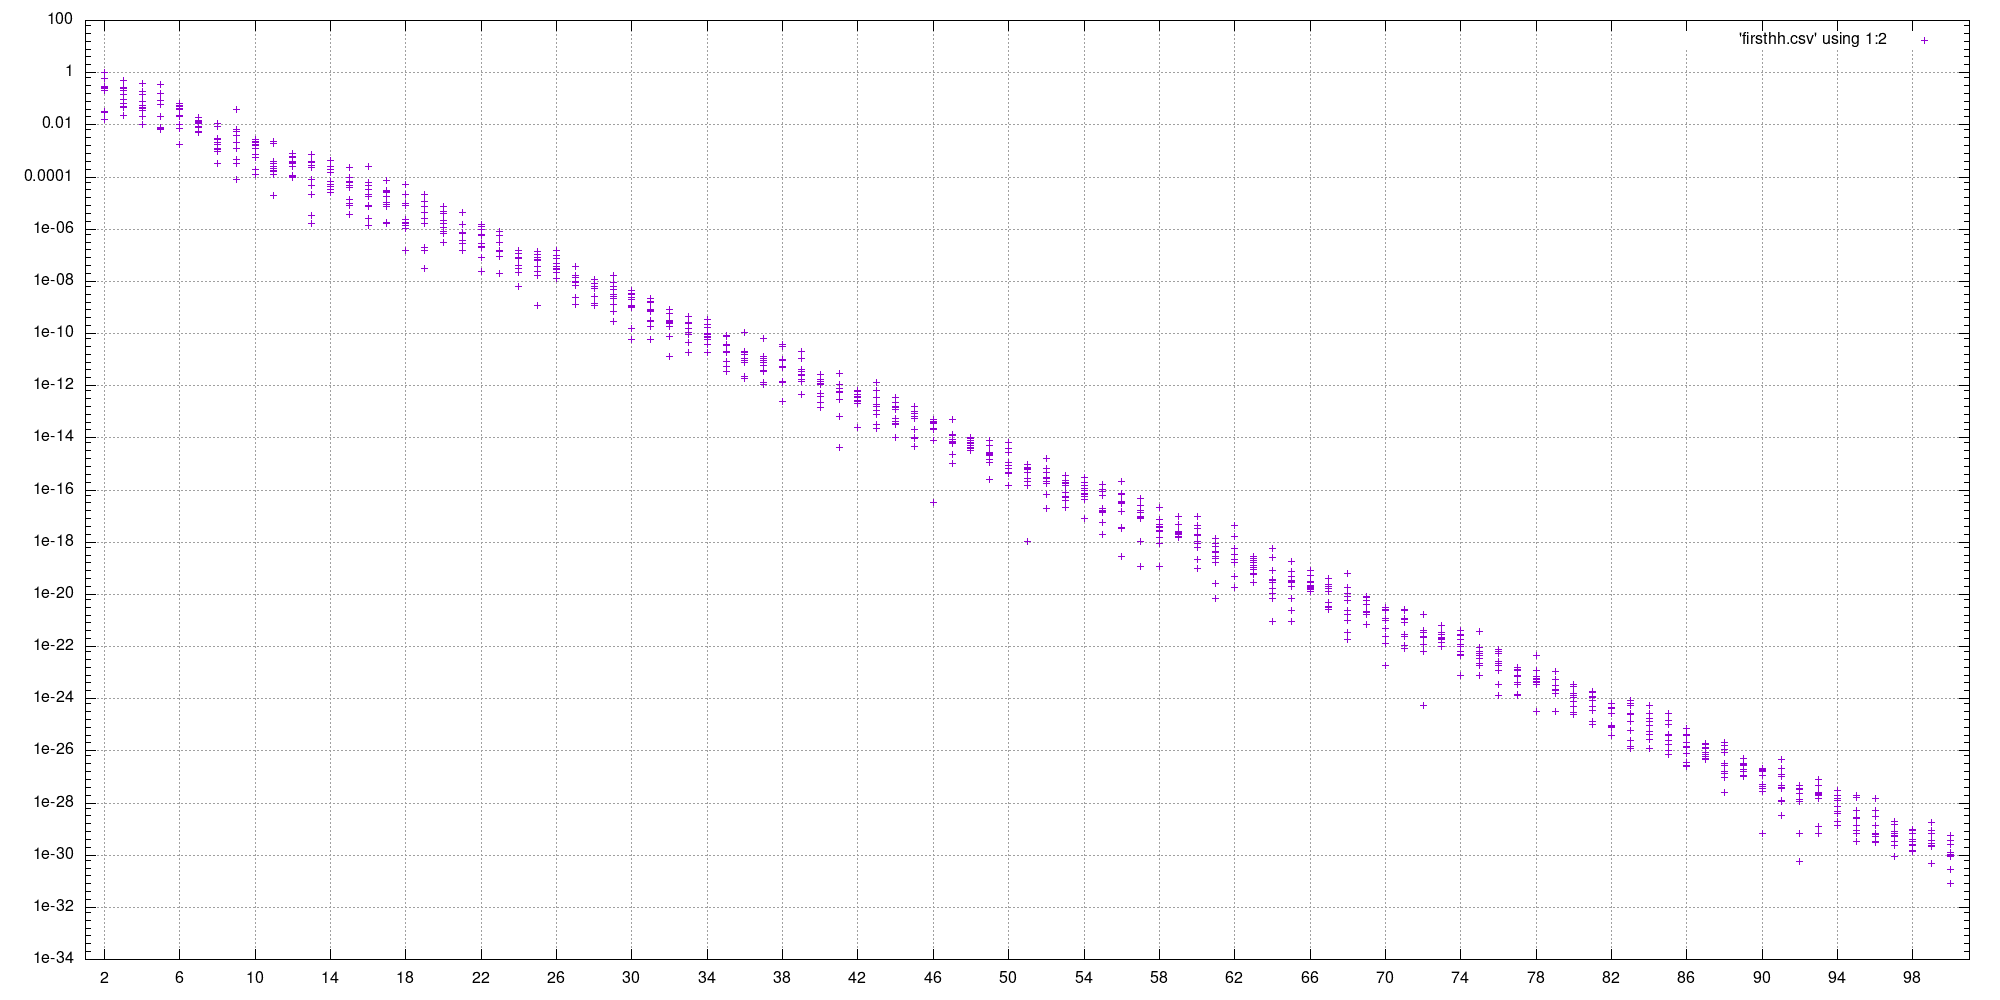
\includegraphics[width=\linewidth]{../../src/firsthh.png}
\centering
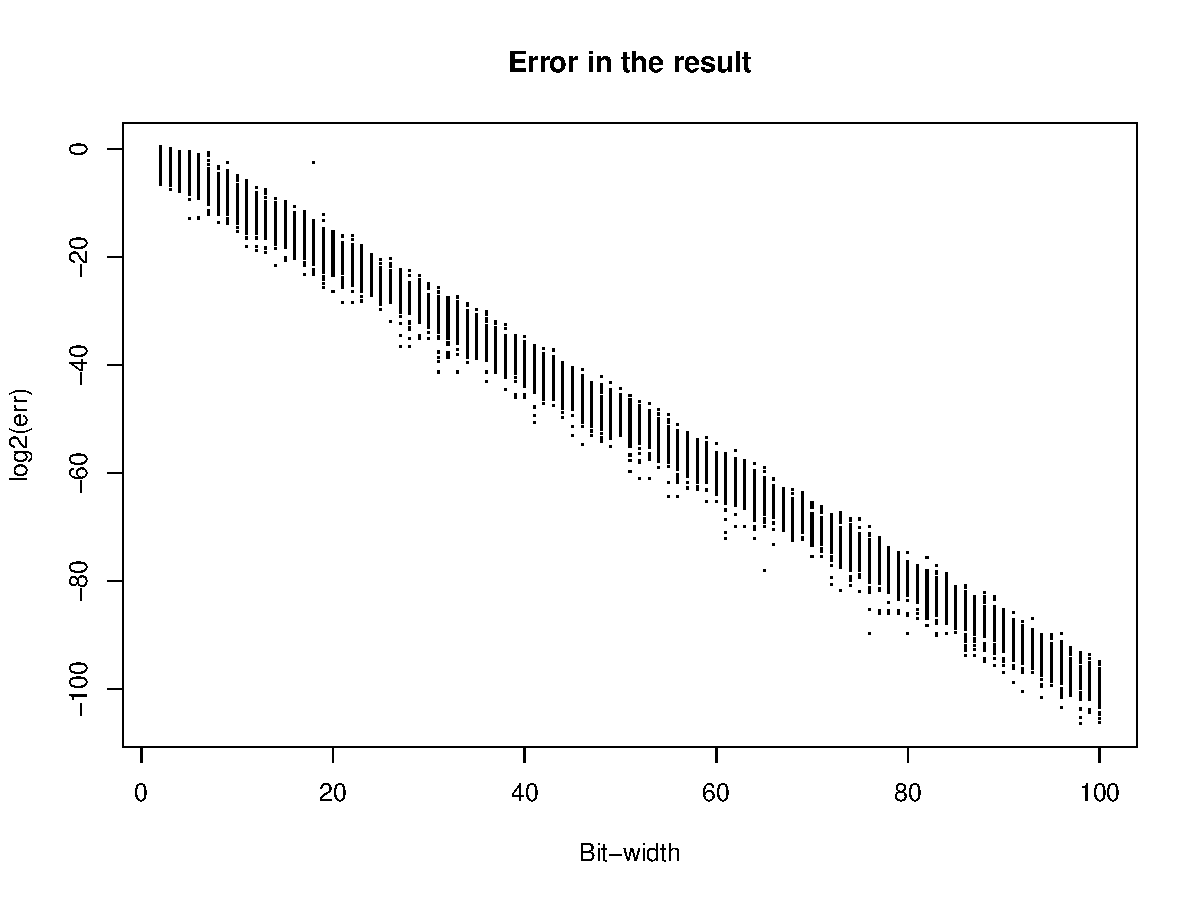
\includegraphics[scale=0.55]{../../src/err.pdf}
\end{adjustwidth}

\end{frame}

%------------------------------------------------

\begin{frame}
%\frametitle{Results of the experiment}

\begin{adjustwidth}{-2em}{-2em}
%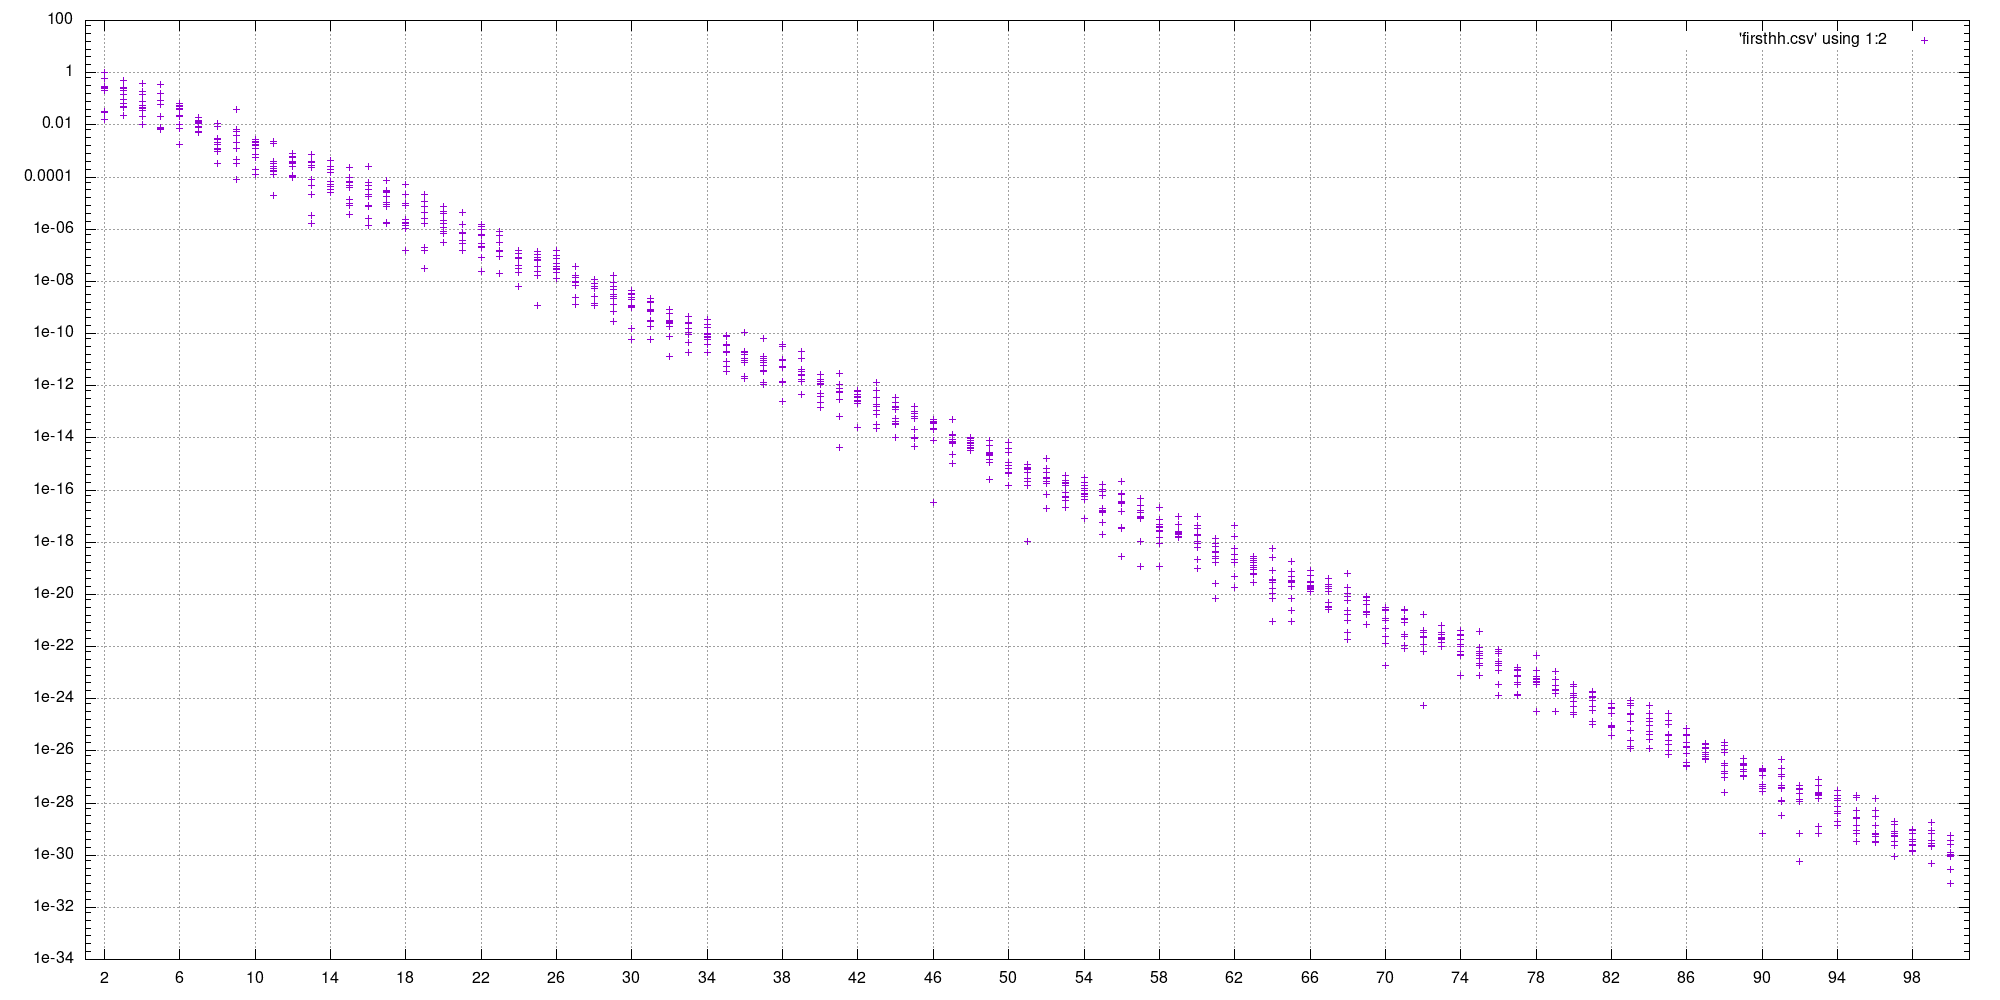
\includegraphics[width=\linewidth]{../../src/firsthh.png}
\centering
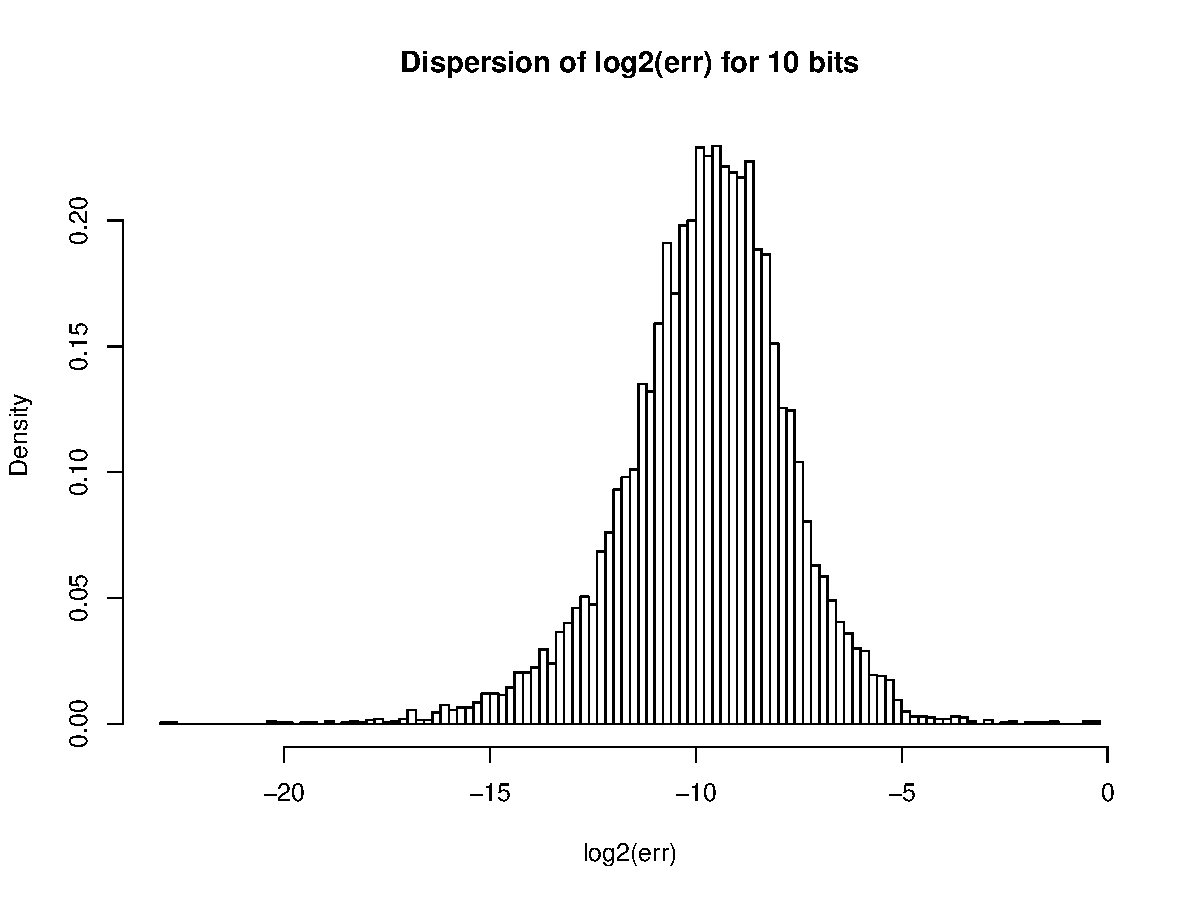
\includegraphics[width=\linewidth]{../../src/err10.pdf}
\end{adjustwidth}

\end{frame}

%------------------------------------------------

\begin{frame}
%\frametitle{Results of the experiment}

\begin{adjustwidth}{-2em}{-2em}
%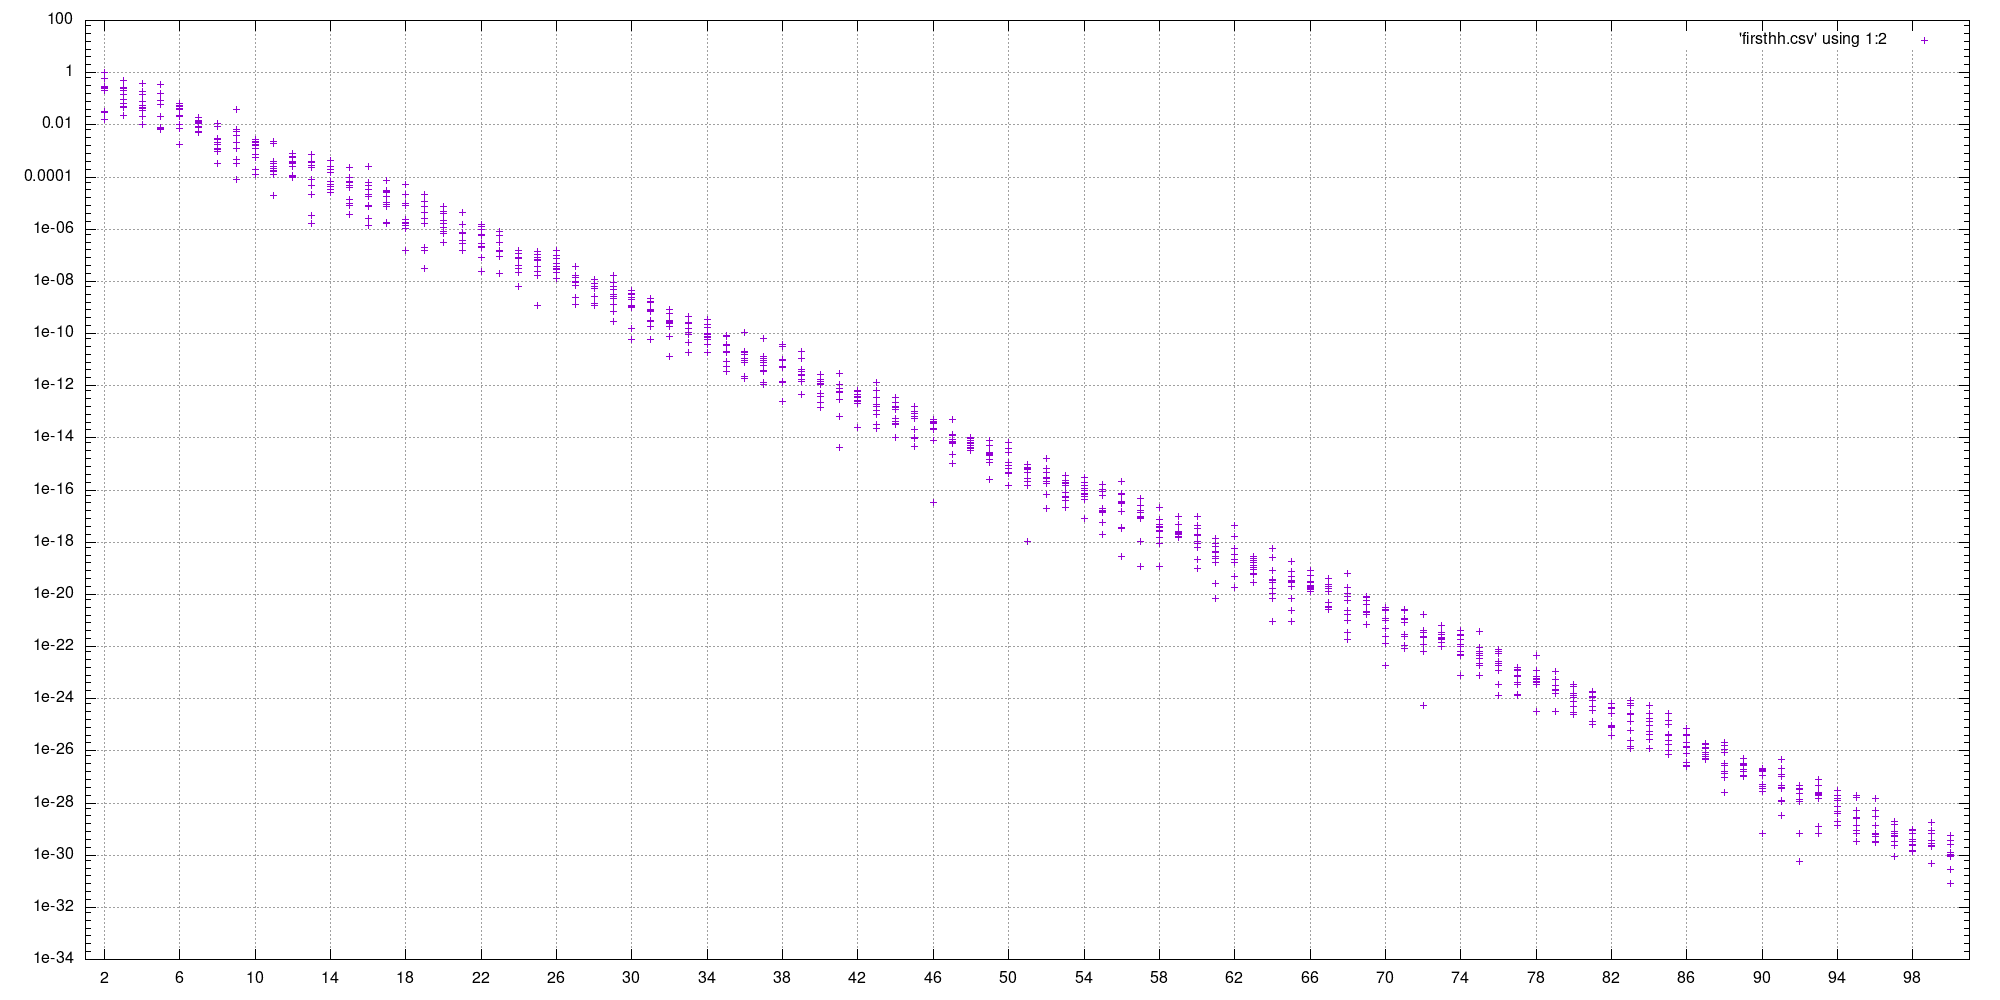
\includegraphics[width=\linewidth]{../../src/firsthh.png}
\centering
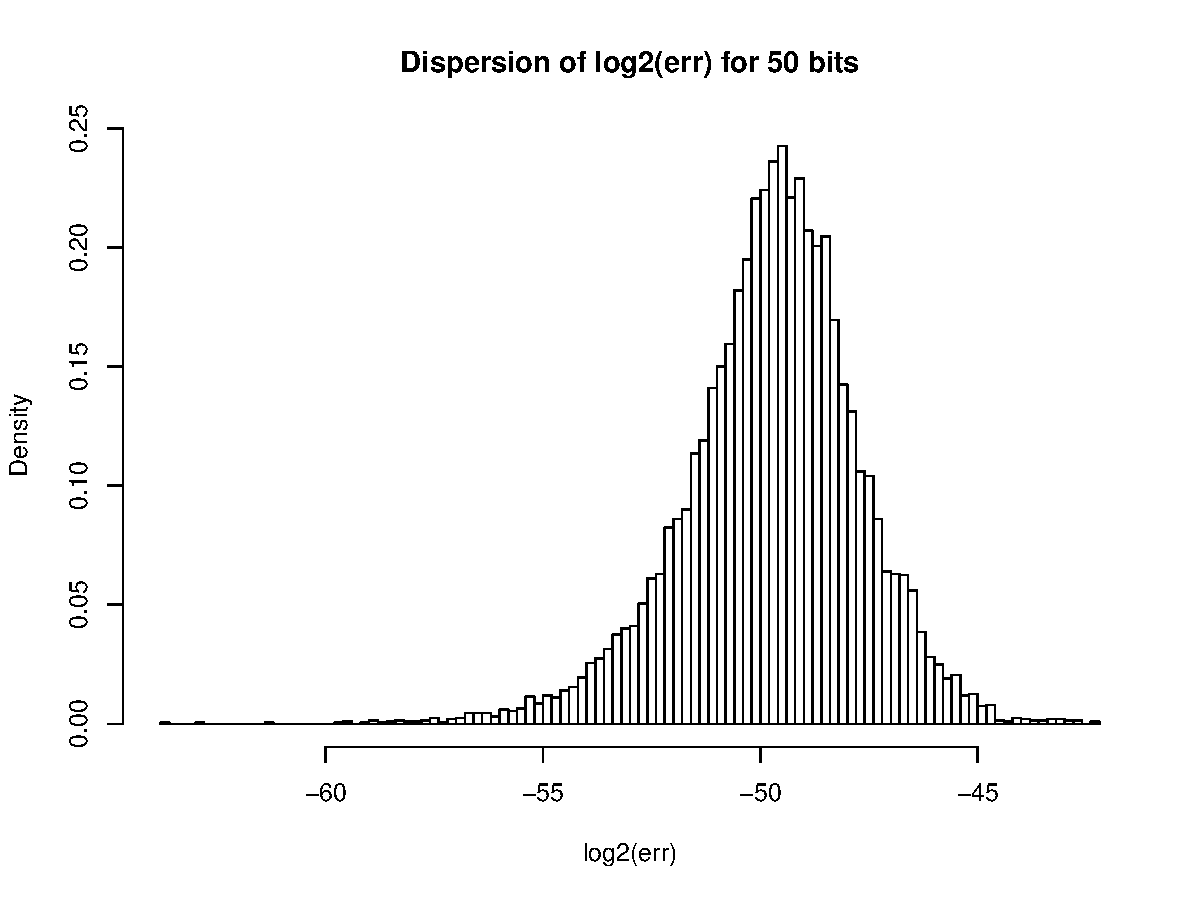
\includegraphics[width=\linewidth]{../../src/err50.pdf}
\end{adjustwidth}

\end{frame}

%------------------------------------------------

\begin{frame}
%\frametitle{Results of the experiment}

\begin{adjustwidth}{-2em}{-2em}
%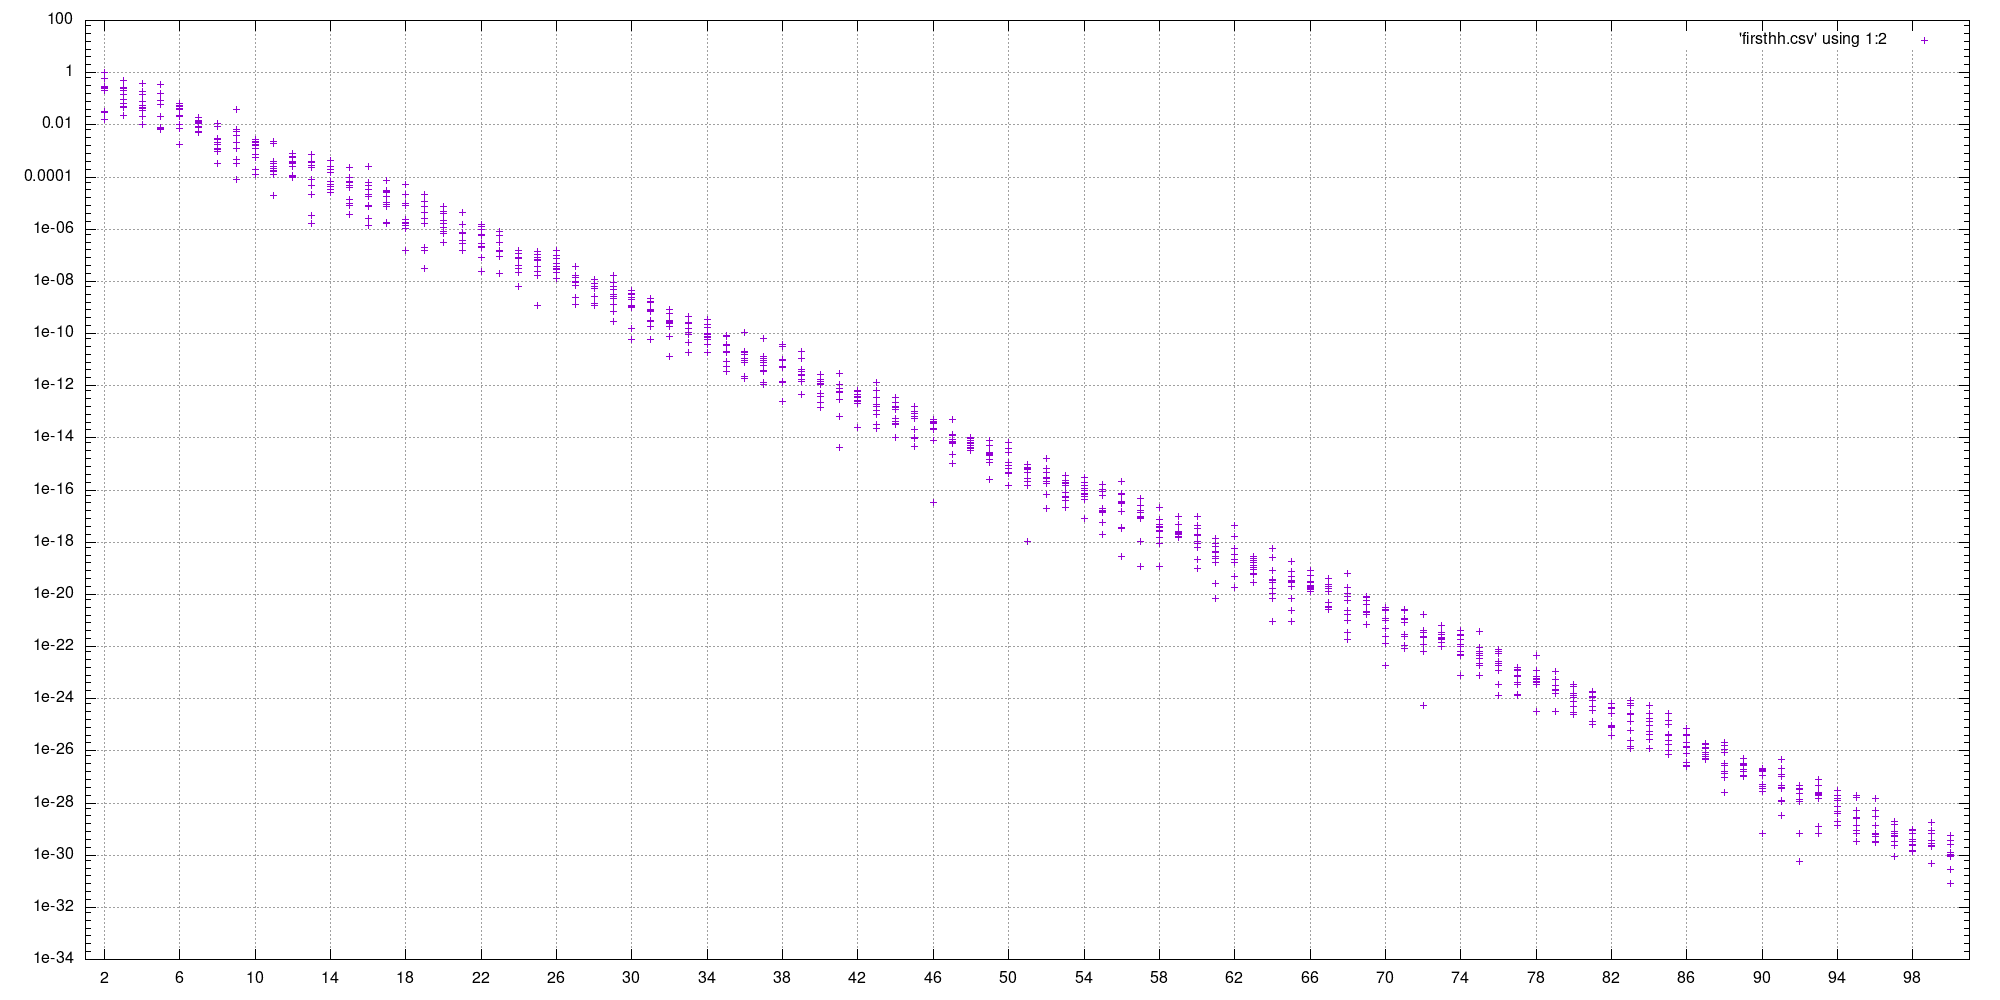
\includegraphics[width=\linewidth]{../../src/firsthh.png}
\centering
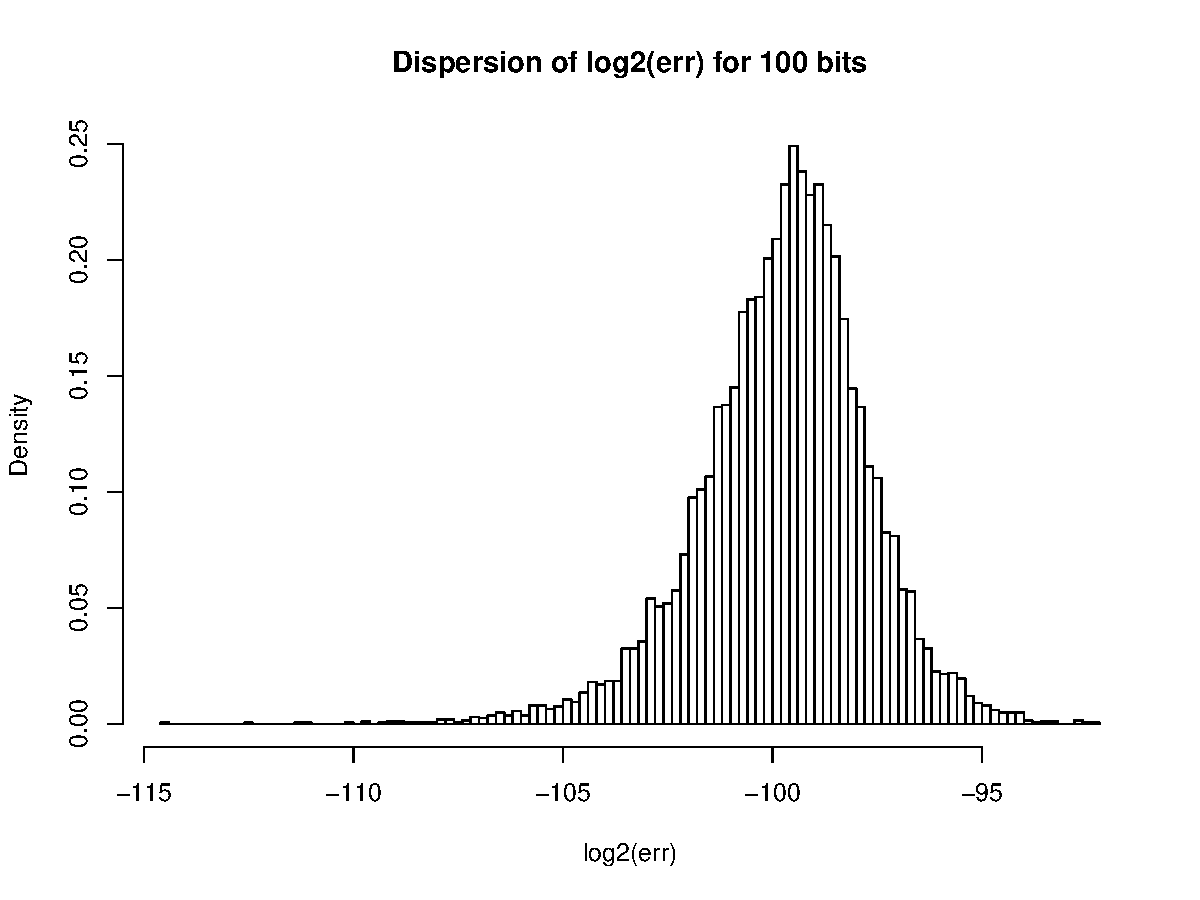
\includegraphics[width=\linewidth]{../../src/err100.pdf}
\end{adjustwidth}

\end{frame}

%------------------------------------------------

\begin{frame}
\frametitle{Observations}
Let $\epsilon_b$ be the error in the result with width $b$, then the following 
hypothesis can be proposed:
\begin{itemize}
\item The mean of $\log_2(\epsilon_b) \approx -b$.
\item The standard deviation $\approx 2$.
\end{itemize}

\end{frame}

%------------------------------------------------

\begin{frame}
\frametitle{Skip modifications}

\begin{itemize}
\item The modification of the Householder algorithm to add a custom bit-width 
can be almost avoided using C++.

\item The MPFR C++ library, uses a wrapper to replace automatically all the 
operations with the custom bit-width arithmetic.

\item However, the documentation is almost inexistent, and not all capabilities 
are available.
\end{itemize}
\end{frame}

%------------------------------------------------

\begin{frame}
\frametitle{Future steps}

\begin{itemize}
\item Test the hyphothesis for the current results.
\item Perform experiments in Householder with different precision in the 
variables.
\item Determine how to use the MPFR wrapper to avoid modifications.
\end{itemize}

\end{frame}

%------------------------------------------------

\begin{frame}
\frametitle{Possible application}

PCA can be applied to satellite images:

\begin{itemize}
\item Satellites have different bands, so different layers of the same region 
are obtained.
\item Those layers are correlated, and PCA can extract the main information in 
only a few uncorrelated layers.
\item \textbf{Example:} from 6 bands, PCA could extract 99.3\% of variance in 
only 3 layers.
\end{itemize}

\begin{tabular}{l l l l l l l}
Component & 1 & 2 & 3 & 4 & 5 & 6 \\
\hline
Percentage & 88.82 & 17.62 & 2.94 & 0.38 & 0.18 & 0.05 \\
\end{tabular}

\end{frame}

%------------------------------------------------

\begin{frame}
\frametitle{Possible application}

\begin{figure}[h]
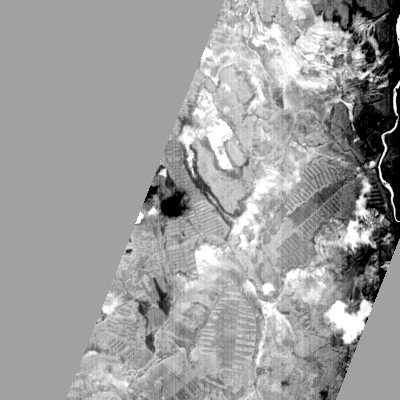
\includegraphics[width=0.45\textwidth]{pca1}
\hspace{1em}
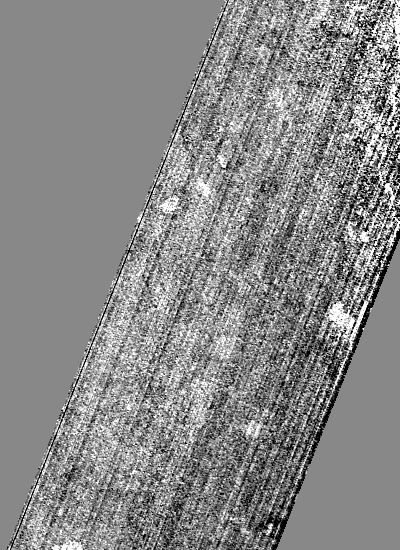
\includegraphics[width=0.45\textwidth]{pca20}
\caption{The first component (left) carries almost all the information, while 
the 20 component (right) is almost noise.}
\end{figure}

\end{frame}

\end{document}
